\chapter{Turing Machine}
\label{ch-turing}

\newcommand{\TA}[0]{\Sigma^+}

This chapter is based on Ref.\cite{wiki-turing-machine}.

A {\bf Turing Machine} (TM)  can be explained as a 
special case of a Petri net (pnet), and that
is the approach that we take in this chapter.
Petri nets are discussed in Chapter \ref{ch-petri}. We will assume
that the reader has read that chapter before tackling this one.

In fact, a TM can be viewed as a generalization
of a special case of a Petri net called a Finite
State Machine (FSM).  FSM are discussed
in Chapter \ref{ch-finite-state}.
We will assume
that the reader has read that chapter too before tackling this one.

Fig.\ref{fig-turing-phsical} is
a diagram of the components
of a TM, if one were to build one.
It consists of a 
\begin{itemize}
\item
a {\bf tape}. The tape is infinite in both directions,
but only a finite number of tape cells may be non-blank.
\item
a {\bf head}
that is one tape cell wide. It moves, relative to the tape,  from one tape cell, 
to the cell immediately to its right or to its left.
The head can read the value of the symbol under it and replace
it (write) by another symbol.
\item {\bf control/memory} unit that remembers 
the current place/state ($\rvp_2$ in Fig.\ref{fig-turing-phsical})
\end{itemize}

\begin{figure}[h!]
\centering
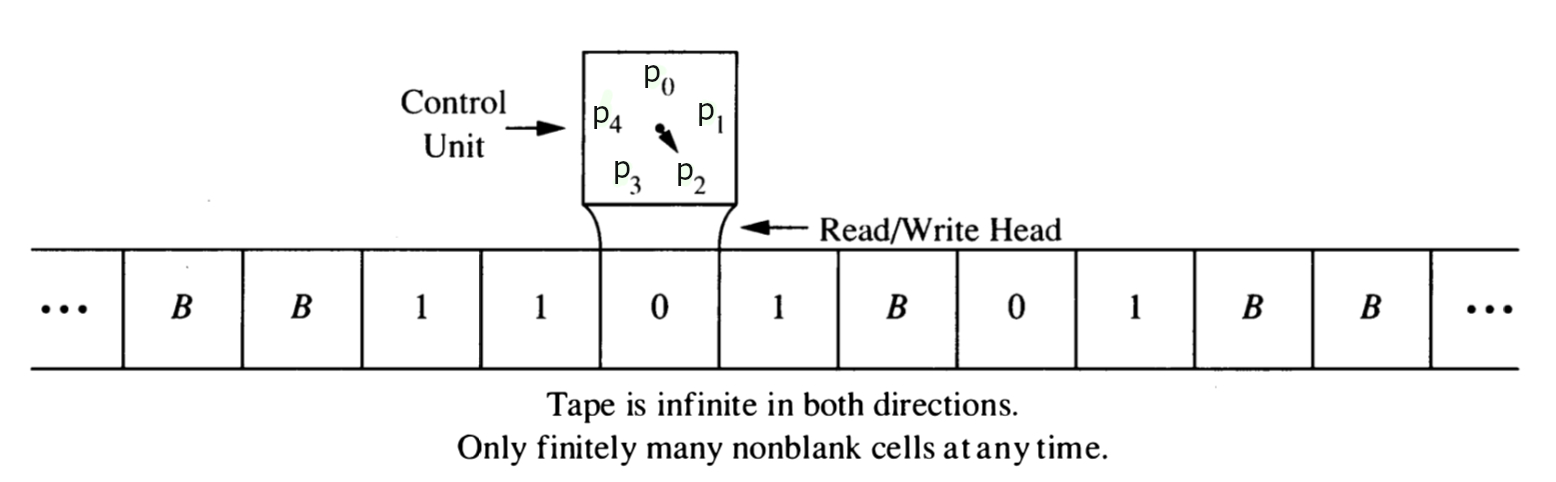
\includegraphics[width=6in]
{turing/turing-physical.jpg}
\caption{Turing Machine if one were to build one.}
\label{fig-turing-phsical}
\end{figure}

\section{Example}

\begin{figure}[h!]
$$
\begin{array}{cc}
\xymatrix@C=6pc@R=3pc{
\PinkCircle{\rva}
\ar[rr]|{\rvx_1=(0,P,R)}
\ar[rd]|{\rvx_3=(1,P, L)}
&&\Circle{\rvb}\ar@(ru,lu)[]_{\rvx_6=(1,P,R)}
\ar@/_2pc/[ll]|{\rvx_2=(0,P,L)}
\\
\ar[u]
&\Circle{\rvc}
\ar[ru]|{\rvx_4=(0,P, L)}
\ar[r]|{\rvx_5=(1,P, R)}
&\DCircle{\rvh}
}
&
\begin{array}{c|c|c|}
\rvp\rarrow \rvx
&\ket{\rvp'}=\rvx\ket{\rvp}
& \lam=(\lam_r,
\lam_w,
\lam_m)
\\
\hline\hline
\rva\rarrow\rvx_1
&\rvb
&(0,P,R)
\\ \hline
\rvb\rarrow\rvx_2
&\rva
&(0,P,L)
\\ \hline
\rva\rarrow\rvx_3
&\rvc
& (1,P,L)
\\ \hline
\rvc\rarrow\rvx_4
&\rvb
& (0,P,L)
\\\hline
\rvc\rarrow\rvx_5
&\rvh
&(1,P,R)
\\ \hline
\rvb\rarrow\rvx_6
&\rvb
&(1,P,R)
\\ \hline
\end{array}
\end{array}
$$
\caption{The \qt{3-state busy beaver} Turing machine represented as a FSM Petri net.}
\label{fig-3-state-bb}
\end{figure}

Fig.\ref{fig-3-state-bb} shows an example of
a TM represented as a FSM Petri net. Everything in this diagram
should be familiar after reading the chapters
on pnets and FSM, except for the
transition  labelling function $\lam()$.

Whereas $\lam$ is a scalar (i.e., an element of the alphabet $\Sigma$)
for a FSM, for a TM its a triple $(\lam_r, \lam_w, \lam_m)$.
$\lam_r$ is the tape symbol read, $\lam_w$
is the tape symbol written (after erasing the 
previous one). $\lam_m\in\{R, L\}$
commands the head to move one cell to the right (R)
or to the left (L).



\section{Precise Definition}

\hrule
Same as in FSM:

$\calx =\{\rvx_i\}_{i=1}^{nx}$ are the {\bf transition nodes} of the pnet.

$\calp =\{\rvp_i\}_{i=1}^{np}$ are the {\bf place (or state) nodes} of the pnet.

$\rvp(0)\in \calp$, {\bf starting place }

$\calp_{acc}\subset \calp$ are the 
{\bf acceptor places}

$\Delta:\calx\times\calp\rarrow \calp$ is the 
{\bf transition function}
\hrule
New for TM

$HALT\in \calp_{acc}$

$\TA =$ {\bf tape alphabet}

$B\in \TA$ {\bf blank space}.

$\Sigma=$ {\bf input alphabet}. $\Sigma\subset\TA-\{B\}$. 

$\lam_{r}:\calx\rarrow \TA$ {\bf read symbol assigning function}

$\lam_{w}:\calx\rarrow \TA$ {\bf write symbol assigning function}

$\lam_{m}:\calx\rarrow \{L,R\}$ {\bf move command
assigning function}

$\lam = (\lam_r, \lam_w, \lam_m)$ is the
{\bf transition labelling function}

$\lam_\rvp: \calx(\rvp\rarrow)\rarrow \TA$ is the
{\bf restriction of $\lam()$ to $\calx(\rvp\rarrow)$}

\hrule
$\Phi_{TM}=\av{\Phi_{pnet},\calp_{acc}, \Sigma,
\Sigma^+, \lam, \Delta}$



